\glsresetall

Following the \emph{Engineering Design Process}, the initial objectives
need to be clarified before searching for the solution principles.
For this purpose, we performed a literature review to identify the
state of the art.

We summarize in this chapter the stages and results of the
\emph{Systematic Mapping of the Literature}, a process described in section~\ref{sec:method_literature_review}.

Since the \emph{Engineering Design Process} is iterative and includes feedback loops, in
section~\ref{sec:mapping/overview}, we estate the objectives of the
\emph{original} literature mapping. These objectives were later refined,
incorporating the results of this study.
In section~\ref{sec:mapping/method}, we describe our method.
In section~\ref{sec:mapping/results}, we summarize the results of the literature mapping.
Finally, in section~\ref{sec:mapping/discussion}, we discuss the interpretation of our findings
and insights.

The content of this chapter appears in the article \emph{Interactive Data Exploration
of Distributed Raw Files: A Systematic Mapping Study}~\cite{Alvarez2019},
published on IEEE Access.

\section{Overview}
\label{sec:mapping/overview}
\gls{IDE} tools target the Data Understanding phase of \gls{CRISPDM}. They have
human intuition as a core part of the process, where the user tentatively
explores the data, iterating and reformulating the queries as
their knowledge and insight change with each iteration.

A system that can be used in such a way needs to be lightweight, adaptive
and have reasonably low response times---\cite{Miller1968} considers two seconds
to be the upper limit for the continuity of thoughts---,
helping and assisting without getting in the way of the person involved in
the loop.

Because of this exploratory nature, early decisions on data structure,
storage, and indexing are inappropriate~\cite{Kersten2011}. They introduce latency
and optimize for a pattern that only happens for a brief period.

This problem can be tackled at different levels---from the physical layout on disk
to the interface interacting with the user. In 2015, Idreos~\cite{Idreos2015}
classified several of these solutions depending on which approach they take
on the issue. This paper originally attracted our attention  due to the potential
applications in \gls{HEP}\footnotemark, although
the techniques found can be of interest to other scientific domains.

\footnotetext{
    This research was initiated while employed at \gls{CERN},
    so \gls{HEP} was the original target use case.
}

In summary, we need to satisfy three main requirements:

\begin{enumerate}
  \item \emph{Interactive response times}, as already discussed
  \item \emph{Access to raw data files}. Pre-loading data in main memory is not an
    option due to the data volume and because we aim for a system that extends and does
    not replace the existing data management solution
  \item Ideally, \emph{distributed}, since files are stored and replicated by an already existing
    distributed storage system~\cite{Baud2012}.
\end{enumerate}

The granularity of the access has to be higher than \emph{file level} because
scientists normally care about datasets that are defined by the data origin,
year, conditions, etc\ldots, and one dataset may be distributed across
several files.

\section{Method}
\label{sec:mapping/method}

Idreos \etal~\cite{Idreos2015} propose a classification of different possible approaches
to our problem.
This study provides an excellent introduction but we wanted to expand on it by answering
two questions that were not covered by the original paper and we also wished to survey
the subsequent evolution of the domain.

\subsection{Research questions}
\label{sec:mapping/research_questions}

\subsubsection{RQ1. How has the research area evolved?}
Given that this is an active research area, it has probably progressed since
the tutorial that we are using as a baseline. Therefore, the first
question to answer to decide how to focus future research is:
How has it evolved since 2015?

\subsubsection{RQ2. What is the maturity level of the research area?}
How many complete and reliable solutions are available?
Are they successfully implemented in practice?
How do they improve the users' experience? Identifying publications is not enough,
we also want to assess in what part of the software life-cycle they focus.

\subsubsection{RQ3. How far are we from a tool that solves our three requirements?}
The final target of this research is to identify solutions that cover our three
requirements.
Even though Idreos closed their tutorial by
mentioning the importance of interconnection research~\cite{Idreos2015}, they do not provide
any references or study on this area.

\subsection{Search strategy}
\label{sec:mapping/search_strategy}

For the retrieval of studies, it is necessary to clearly define
how the search is going to be performed. This work combines
three different strategies, as follows:

\begin{itemize}
  \item Set of known works obtained from \cite{Idreos2015} because our RQ2 is
    not covered by the original classification.
  \item Forward snowballing~\cite{Webster2002} from the known set of publications using Google Scholar.
  \item For completeness, database searches to improve the coverage of our study.
\end{itemize}

Jalali and Wohlin~\cite{Jalali2012} argue that snowballing and database searches
can lead to similar patterns but they also agree that it is
``not easy to draw any general conclusions'' about if the conclusions obtained are the same
using the two different approaches. Thus, we have opted to follow both.

The set of digital libraries consulted is:

\begin{itemize}
  \item ACM Digital Library
  \item Elsevier (Science Direct)
  \item Springer
  \item IEEE Digital Library
  \item Wiley Online Library
  \item World Scientific Net
\end{itemize}

Given the fast pace at which the field moves, older papers have been probably
superseded or, if still relevant, we expect them to be already included in \cite{Idreos2015}.
Consequently, we have limited the scope in time to studies published from 2010 onwards.

All of the references obtained by any of the previous method were imported into
a group in the \emph{Mendeley Reference Manager}. Any obviously non-interesting entry
---such as book or proceeding indexes---were removed at this stage.
The definitive list can be found on a public group in
\href{https://www.mendeley.com/community/interactive-data-exploration-in-science-systematic-mapping/}{Mendeley.com} and in
\href{https://www.zotero.org/groups/4517638/interactive-data-exploration-in-science-systematic-mapping/library}{Zotero.com}\footnotemark.

\footnotetext{Both groups are
    \texttt{interactive-data-exploration-in-science-systematic-mapping}
}

\subsection{Study selection criteria}
We based the initial screening of studies on title, abstract, and keywords.
In some cases, when the information provided by these fields was
insufficient to take a decision, we also considered their conclusions
or read the complete study.

We have focused here on finding primary studies related to data exploration.
The filtering was performed using the following exclusion criteria:

\begin{itemize}
  \item \emph{Unsupported language} Studies written in a language different than
  English, Spanish or French
  \item \emph{Incomplete publication} Abstract only, or presentations were excluded
  \item \emph{Off topic} Out of the data exploration domain
  \item \emph{Not a primary study} Secondary, tertiary and surveys
  \item \emph{Duplication} In case of duplication or high similarity for the same
  set of authors, only the most complete or the most recent was
  taken into account.
\end{itemize}

Those publications that passed the inclusion criteria were reviewed to make
sure all their fields were correct. Normally, this should have been done during
the previous stage but due to the sheer volume of publications yielded by the
search strategy this step was postponed until the filtering was done. Because only
title and abstract were used for the filtering, this did not affect the end
result.

\subsection{Classification}
Publications that pass the selection criteria will be classified into two axes:
data exploration facet and research type.

\subsubsection{Category}
\label{sec:mapping_category}
As mentioned in section~\ref{sec:mapping/research_questions}, we base our study on
the classification done by Idreos \etal~\cite{Idreos2015}, which is included for
convenience in table~\ref{tab:mapping/clustering}. For more details, we refer the
interested reader to Idreos' tutorial.

For our purposes, we have assigned one single category to each work covered
by our study, choosing the most prominent topic when more than one category
could fit.

\begin{table}[hptb]
  \footnotesize
  \begin{tabularx}{\textwidth}{>{\hsize=10.5em}X X X X}
    \hline
    \multicolumn{4}{l}{\textbf{User Interaction}} \\
    \hline
    \textit{Data Visualization} & Visual Optimizations & Visual Tools & \\
    \textit{Exploration Interfaces} & Automatic Exploration & Assisted Query Formulation & Novel Query Interfaces \\
    \hline
    \multicolumn{4}{l}{\textbf{Middleware}} \\
    \hline
    \textit{Interactive Performance Optimizations} & Data Prefetching & Query Approximation & \\
    \hline
    \multicolumn{4}{l}{\textbf{Database Layer}} \\
    \hline
    \textit{Indexes} & Adaptive Indexing & Time Series & Flexible Engines \\
    \textit{Data Storage} & Adaptive Loading & Adaptive Storage & Sampling \\
  \end{tabularx}
  \caption{Categories of Interactive Data Exploration solutions}\label{tab:mapping/clustering}
\end{table}

\subsubsection{Research type}
To answer our second research question---the maturity of the area---we follow
the classification of research approaches done by \cite{Wieringa2006},
as our guidelines for systematic mapping do~\cite{Petersen2007}.

We summarize the different research types in table~\ref{tab:mapping/research_type}.

As per this classification, we expect mature solutions that have been
implemented in practice to be covered by one or more \emph{Evaluation Research}
studies. If, on the contrary, they are on very early stages, then most
related studies will fall into the \emph{Philosophical} or
\emph{Opinion} categories.

\begin{table}[hptb]
  \small
  \begin{tabularx}{\textwidth}{l >{\raggedright\arraybackslash}X}
    \hline
    \textbf{Research type} & \textbf{Description} \\
    \hline
    \textit{Evaluation research} & Investigation of a problem or implementation in practice. \\
    \textit{Proposal of solution} & These papers propose a solution and argue for its relevance without
      complete validation. A proof-of-concept may be offered. \\
    \textit{Validation research} & These papers investigate the properties of a solution proposal that
      has not yet been implemented in practice. \\
    \textit{Philosophical papers} & These papers sketch a new way of looking at things, a conceptual
      framework, etc. \\
    \textit{Opinion papers} & These paper contain the author's opinion. \\
    \textit{Personal experience papers} & These paper should contain a list of lessons learned by the
      author from his or her own experience. The evidence can be anecdotal. \\
  \end{tabularx}
  \caption{Research type for the Systematic Mapping}\label{tab:mapping/research_type}
\end{table}

\subsection{Data extraction and visualization}
At this stage, the papers were filtered and classified. We needed to summarize
the obtained data in a way that is useful to answer our research questions.

To answer \emph{RQ1}, we focused on the counting of each category
and their visualization on a time series plot.

To answer \emph{RQ2}, a bubble plot can help to more easily identify
the most frequent research type per category. In this way, we can identify if
one area is more mature than other. Additionally, we also counted and displayed
how many publications include some sort of user study, which should prove
if any particular solution is successful at improving the integration of a
human on the loop.

Finally, for \emph{RQ3}, we flag interesting papers classified under
\emph{Proposal of Solution} with the three requirements separately, if stated
on their abstract or conclusions.

Additionally, while it was not in the original research questions, we can
also extract which publication forums are the most prominent on our results.

\section{Results}
\label{sec:mapping/results}
In this section, we describe the outcome of each stage of the systematic mapping.

\subsection{Study selection}
As previously described, we have three different sources of papers:
the references from \cite{Idreos2015}, search engines, and forward snowballing
from those that pass the selection criteria.

Table \ref{tab:mapping/searches} displays the search queries that were used for
each digital library.
All searches were done on May 16, 2017 and they yielded a total of \numprint{5 525} articles.

Idreos' tutorial provided 47 papers and the forward snowballing provided 116.

From this total of \numprint{5 688}, only \numprint{242}---4.25\%--were accepted, the details are
shown in table \ref{tab:mapping/acceptance}. This rather low hit ratio
comes mostly from the on-line searching of digital libraries
because the lack of well defined, or univocal, keywords makes it difficult to decide what
to search for. We do not seem to be alone in this respect~\cite{Kitchenham2013,Jorgensen2007}.

Even once defined, and because we must use different search engines, there are
few or no commonalities between the way queries can be written and handled
between different archives~\cite{Bailey2007, Brereton2007}.

This yield is no smaller than those of systematic studies in
other fields, which can be as low as 0.3\%~\cite{Oakley2003}.

\begin{table}[hptb]
  \small
  \begin{tabularx}{\textwidth}{l X X} \hline
    \textbf{Library} & \textbf{Scope} & \textbf{Search} \\ \hline
    ACM Digital Library & Full text & \texttt{("RAW data" OR "RAW file" OR "ROOT file") AND (query OR exploration)} \\
    ScienceDirect & Title, abstract, keywords (computer science) & \texttt{((RAW OR ROOT) AND (query OR exploration))} \\
    Springer & Full text (computer science) & \texttt{("RAW data") AND (query OR exploration) + ("RAW file") AND (query OR exploration)} \\
    Wiley Online Library & Abstract & \texttt{RAW AND query} \\
    IEEE Digital Library & Abstract & \texttt{RAW AND query} \\
    World Scientific Net & Full text (computer science) & \texttt{RAW AND query} \\
  \end{tabularx}
  \caption{Queries used to obtain the first set of articles for the Systematic Mapping}\label{tab:mapping/searches}
\end{table}

\begin{table}
    \small
    \begin{tabularx}{\textwidth}{r r r r r r} \hline
    \bf Accepted & \bf Duplicated & \bf Not Primary & \bf Off Topic & \bf Too Old & \bf Total \\ \hline
    242 & 9 & 16 & \numprint{5 295} & 126 & \numprint{5 688} \\
    \numprint[\%]{4.25} & \numprint[\%]{0.16} & \numprint[\%]{0.28} & \numprint[\%]{93.09} & \numprint[\%]{2.22} & \numprint[\%]{100}
  \end{tabularx}
  \caption{Accepted and rejected papers count}\label{tab:mapping/acceptance}
\end{table}

\subsection{Study data extraction}

Table \ref{tab:mapping/category_summary} displays the frequency of publications for each
classification cluster proposed by Idreos~\cite{Idreos2015}. It is worth mentioning that
four papers on the \emph{Database Layer} did not fall into
the predefined clusters, given their genericity~\cite{Kersten2011}, or as an
evaluation of different techniques~\cite{Siddiqa2017,Zoumpatianos2015,Palpanas2015}.

Figure \ref{fig:mapping/layer_vs_type} displays the frequency of each major cluster
against the research type count for each one. In table~\ref{tab:mapping/publication},
we display the publication forums where more than one study has been published.
While there are two main forum, summing 30.58\% of all the publications,
most of the papers are spread out on different conferences and journals.

It is worth noting that this table includes gray literature; that is, outside of the
formal academic publishing.
While one may argue that this papers have not been yet subject of a peer
review, they are still included because gray literature can be, and is, a useful
source of knowledge for information users~\cite{Lawrence2015}. In fact,
Kitchenham \etal~\cite{Kitchenham2007} recommended in their guidelines for systematic
reviews to include gray literature in searches.

\begin{table}[hptb]
  \small
  \begin{tabularx}{\textwidth}{X r} \hline
    \textbf{Category} & \textbf{Count} \\ \hline
    \textbf{User Interaction} & \textbf{86} \\
      \hspace{0.5em} Assisted Query Formulation & 28 \\
      \hspace{0.5em} Visual Optimizations & 25 \\
      \hspace{0.5em} Novel Query Interfaces & 14 \\
      \hspace{0.5em} Visualization Tools & 11 \\
      \hspace{0.5em} Automatic Exploration & 7 \\
      \hspace{0.5em} Exploration Interfaces & 1 \\
    \textbf{Middleware} & \textbf{48} \\
      \hspace{0.5em} Query Approximation & 34 \\
      \hspace{0.5em} Data Prefetching & 14 \\
    \textbf{Database Layer} & \textbf{108} \\
      \hspace{0.5em} Adaptive Indexing & 26 \\
      \hspace{0.5em} Flexible Engines & 16 \\
      \hspace{0.5em} Time Series & 16 \\
      \hspace{0.5em} Sampling & 15 \\
      \hspace{0.5em} Adaptive Storage & 14 \\
      \hspace{0.5em} Adaptive Loading & 10 \\
      \hspace{0.5em} Spatial Query & 6 \\
      \hspace{0.5em} Other & 5
  \end{tabularx}
  \caption{Frequency of \glsentrylong{IDE} papers by category}\label{tab:mapping/category_summary}
\end{table}

\begin{figure}[hptb]
    \centering
    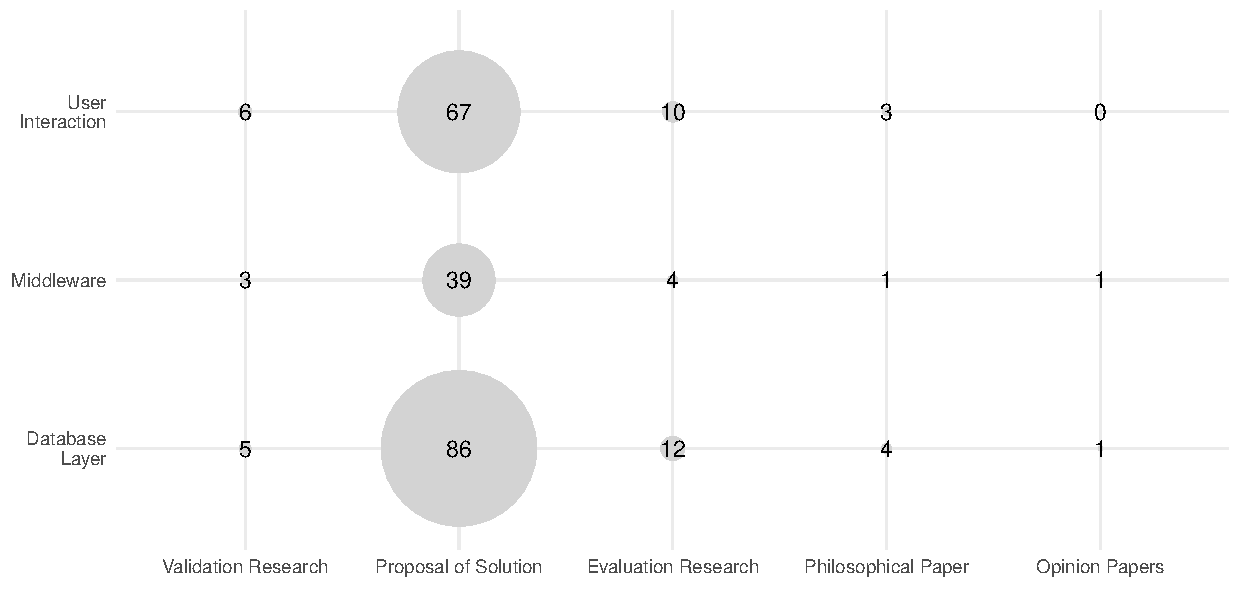
\includegraphics[width=\textwidth]{images/3_mapping/layer_vs_type}
    \caption{\glsfmtlong{IDE} Layer vs Study research type}
    \label{fig:mapping/layer_vs_type}
\end{figure}

\begin{table}[hptb]
  \small
  \begin{tabularx}{\textwidth}{X r} \hline
    \textbf{Publication} & \textbf{Count} \\ \hline
    \textbf{Journal} & \textbf{55} \\
      \hspace{0.5em} The VLDB Journal & 11 \\
      \hspace{0.5em} IEEE Transactions on Knowledge and Data Engineering & 3 \\
      \hspace{0.5em} IEEE Transactions on Visualization and Computer Graphics & 3 \\
      \hspace{0.5em} International Journal of Cooperative Information Systems & 3 \\
      \hspace{0.5em} Journal of Big Data & 3 \\
      \hspace{0.5em} ACM Transactions on Database Systems & 2 \\
      \hspace{0.5em} Future Generation Computer Systems & 2 \\
      \hspace{0.5em} SIGMOD Record & 2 \\
      \hspace{0.5em} Others & 26 \\
    \textbf{Conference} & \textbf{181} \\
      \hspace{0.5em} ACM International Conference on Management of Data (SIGMOD) & 33 \\
      \hspace{0.5em} Proceedings of the VLDB Endowment & 30 \\
      \hspace{0.5em} IEEE International Conference on Data Engineering & 11 \\
      \hspace{0.5em} Conference on Innovative Data Systems Research (CIDR) & 9 \\
      \hspace{0.5em} Database Systems for Advanced Applications & 5 \\
      \hspace{0.5em} International Conference on Scientific and Statistical Database Management & 5 \\
      \hspace{0.5em} IEEE International Conference on Big Data & 4 \\
      \hspace{0.5em} International Conference on Extending Database Technology & 3 \\
      \hspace{0.5em} International Workshop on Data Management on New Hardware & 3 \\
      \hspace{0.5em} ACM SIGMOD Symposium on Principles of Database Systems (PODS) & 2 \\
      \hspace{0.5em} Advances in Visual Computing & 2 \\
      \hspace{0.5em} Big Data Analytics & 2 \\
      \hspace{0.5em} Database and Expert Systems Applications & 2 \\
      \hspace{0.5em} IEEE International Conference on Mobile Data Management & 2 \\
      \hspace{0.5em} Intelligent Information and Database Systems & 2 \\
      \hspace{0.5em} International Conference on Advanced Cloud and Big Data & 2 \\
      \hspace{0.5em} Workshop on Human-In-the-Loop Data Analytics & 2 \\
      \hspace{0.5em} Others & 62 \\
    \textbf{Gray literature} & \textbf{6}
  \end{tabularx}
  \caption{Frequency of papers by publication forum} \label{tab:mapping/publication}
\end{table}

We refer to our published work~\cite{Alvarez2019} for the complete list of classified publications.

\section{Discussion}
\label{sec:mapping/discussion}

With these results, we now answer the three research questions in
section~\ref{sec:mapping/answers}. Then, in section~\ref{sec:mapping/insights}
we explain the insights we obtain from these answers. Finally,
we enumerate the threats to the validity of this study in
section~\ref{sec:mapping/threats}.

\subsection{Answering the research questions}
\label{sec:mapping/answers}

\subsubsection{RQ1. How has the research area evolved?}
Figure \ref{fig:mapping/layers_histogram} displays the evolution during time
of each of the three major classification clusters: user interaction,
middleware and database.

Considering our search strategy, most of the
results are posterior to 2012. Different approaches seem to be, in general, well
balanced---we refer again to table \ref{tab:mapping/category_summary}---, although there
is space for more works focused on \emph{exploration interfaces} and
\emph{automatic exploration}, which are the less frequent published approaches.

\begin{figure}[hptb]
    \centering
    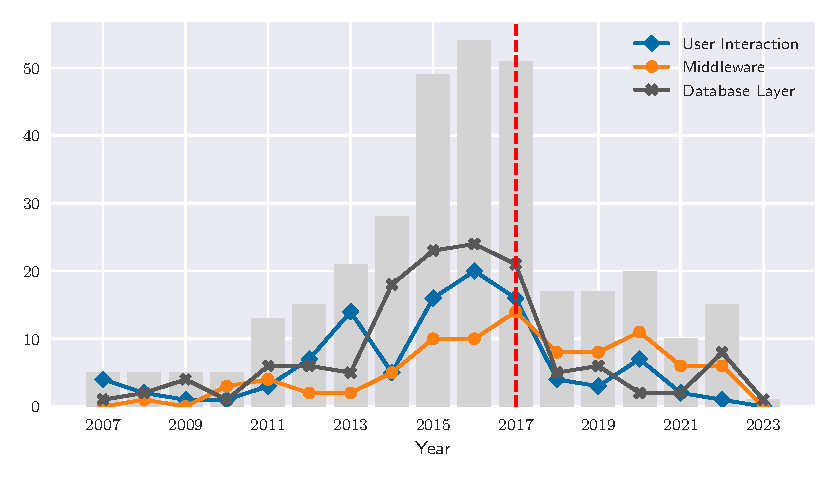
\includegraphics[width=0.6\textwidth]{images/3_mapping/layer_histogram}
    \caption[Number of studies per \glsfmtlong{IDE} layer and year]{
        Number of papers per layer and year.
        Note that the drop during 2017 is because the search was done in May 2017.
    }
    \label{fig:mapping/layers_histogram}
\end{figure}

\subsubsection{RQ2. What is the maturity level of the existing solutions?}
We can use the figure~\ref{fig:mapping/layer_vs_type} to answer this question.
The vast majority of papers considered by this study---79.35\%---fall within the
\emph{proposal of solution} research type.

Meanwhile, \emph{evaluation} and \emph{validation} research are represented
just by a \numprint[\%]{11} and \numprint[\%]{6.07}, respectively.
Only 32 documents (\numprint[\%]{13}) include some sort of user study:
24 for `User Interaction', 4 for `Database  Layer' and 2 for `Middleware'.
Research on how different solutions ---either existing or proposed--- perform in
practice is lacking.

These figures are hardly surprising because they seem to have been commonplace
in computer science for a long time now~\cite{TICHY1995,ZELKOWITZ1997,Sjoberg2005}.
For instance, Sjøberg \etal survey the status of controlled experiments
in software engineering and the numbers they find are equally low, with
only 113 controlled experiments found on \numprint{5 453} papers~\cite{Sjoberg2005}.

It is hard and also out of the scope of this study to make some inferences from these
results. Tichy \etal~\cite{TICHY1995} mention some potential reasons and measures
to improve this situation, namely: difficulty on performing experiments where humans
are involved, the lack of common benchmarks, or even that empirical work is not
encouraged by the journals and conferences of this area.

\subsubsection{RQ3. How far are we from a tool that solves our three requirements?}

\begin{figure}[htbp]
    \centering
    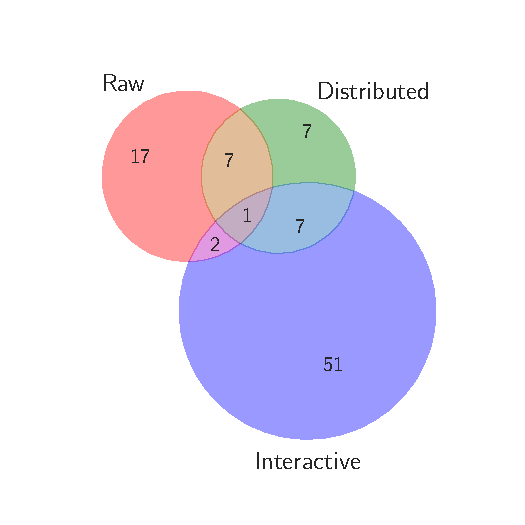
\includegraphics[width=0.5\textwidth]{images/3_mapping/venn}
    \caption{Venn diagram with satisfied initial requirements}
    \label{fig:mapping/venn_requirements}
\end{figure}

In figure \ref{fig:mapping/venn_requirements} we display a Venn diagram with our three
requirements. We can see there is a single study that covers the three requirements:
\textit{{A} {D}istributed {I}n-situ {A}nalysis {M}ethod for {L}arge-scale
{S}cientific {D}ata}, by D.Han \etal~\cite{Han2017}. While they mention the
access over raw files and the fact that it is distributed, they do not
explicitly state anything about their interactivity. However, the measured times
for selective queries that they report are in the order of a few seconds. Consequently, we
decided to consider it to be suitable for interactive usage.

The tests they perform use datasets that are close
to the memory available on the system and, therefore, more tests with bigger dataset sizes
could be needed.

Aside from this paper, no other study combines access to raw data with low
response times.

The solutions that cover at least two out of the three requirements are 
summarized in more detail in section~\ref{sec:mapping/details}.

\subsection{Study insights}
\label{sec:mapping/insights}
Research in data exploration is very active and there has been---and there is---
a myriad of solutions proposed. In fact, this should not come as a surprise:
in 2005 Stonebraker~\cite{Stonebraker2005} had already predicted this was bound to
happen and predicted that there would be an increase of domain-specific tools.
This would explain why, of the all classified studies, only one tool satisfies our
three prerequisites.

In general, several different systems and approaches have been proposed, which could,
perhaps, be seen as building blocks. Not all combinations necessarily make sense
but it seems that there are research opportunities in this direction, depending
on the specific needs to be covered.

For instance, in our particular case, we could consider combining distributed
access over raw files, as Han~\cite{Han2017} does, but using approximate query
processing to reduce the response times.

Code generation is a popular approach for querying raw data files
and approximation aware code generation has been noted as a challenge
that is yet to be addressed~\cite{Mozafari2017AQP}. Consequently, more work on this
particular overlap of approaches may provide interesting results.

On a orthogonal consideration, since the generation of data volume will likely
not slow down, the trend for more tools covering specific
niches is probably going to continue. This diversity of tools is a
challenge in itself in many respects, for example: How do we choose the right solution? What is
the cost of making the wrong choice? What happens if the chosen tool goes
unmaintained in the future and there is no community around it? Will it
be hard to maintain? Of course, these questions are not new in software
engineering but typically there are not many choices when it comes to decide
on traditional data storage systems, such as DBMS.
In the last decade, there has been an increase of available options
(relational, object oriented, schema-less, key-value, \ldots) and, while opting
for a DBMS has become harder, it has remained rather manageable. However, looking at the
results of this study, the difficulty for users to decide will likely become
more challenging.

\subsection{Threats to validity}
\label{sec:mapping/threats}
\subsubsection{Search bias}
The gaps identified may be covered in
journals and conferences associated with the user domain---e.g. astrophysics---,
rather than with computer science and engineering. The forward snowballing
step reduces this risk because these hypothetical publications would most likely
cite the original proposal of solution. However, considering that our research method has
allowed us to find even gray literature, we consider this risk to be low.

\subsubsection{Filtering of articles}
Given the huge number of papers that resulted from the search,
a first filtering was done just based on title and abstract.
This is a difficult challenge. Unlike in other disciplines, sometimes abstracts
do not contain enough information about the paper and keywords can be inconsistent
between journals and authors~\cite{Budgen2008,Brereton2007,Jalali2012}.
As recommended by \cite{Brereton2007}, we have also taken into consideration
the conclusions to cover this issue.

\subsubsection{Classification}
Another concern about these classifications is the bias of the researcher's own
interpretation~\cite{MacLure2005}.
For instance, \emph{Jorgensen and Shepperd} report on a disagreement over
39\% of the reviewed papers in their systematic review~\cite{Jorgensen2007}
due to different interpretations of the description of each category. We
have been careful in this respect to guarantee the internal validity of the
study, although some misclassification may still exist.

Additionally, it can be hard to identify if a solution covers or not one of the
three predefined requirements based just on a paper. They may not have been
explicitly mentioned if the authors did not consider them relevant for the
purposes of their publication. Therefore, there may have been false negatives.

The present paper documents our process and the resulting
publication list has been made publicly available---see
section~\ref{sec:mapping/search_strategy}---, so any interested reader can
replicate and/or validate our results.

\section{Discussion of relevant methods}
\label{sec:mapping/details}
Included for completeness is a summary of each of the nine publications 
that cover, at least, two out of the three requirements.

\subsection{All three requirements}
\newcommand{\scidb}[0]{\textsc{SciDB} }

As already mentioned, the only solution that covers the three requirements is
documented on the paper
\textit{A Distributed In-situ Analysis Method for Large-scale
Scientific Data}~\cite{Han2017}, classified as ``adaptive loading''.

The authors build on top of \scidb~\cite{Stonebraker2011}, a distributed
array-based scientific database, and focus on \textsc{HDF} files~\cite{HDF}.
To avoid the overhead of data pre-loading, they leverage the flexible
architecture of this database engine, providing their own scan operator to read
the data directly from the raw files when needed, which needs to be adapted
to the internal representation of \scidb.

This adaptation is done in two different stages: local and global mapping.

During the local mapping, they read on demand the data that matches the filters 
associated to the query, adapting it to the \scidb chunk representation: pieces 
of array data that are distributed together based on some policy - e.g hashing, 
range partitioning.

At the global mapping stage, the resulting chunks are redistributed across the 
storage nodes following the \scidb policies.

Although not relevant for our use case, it is worth mentioning that they also
merge small files together to reduce the performance penalty of processing many
small files.

This approach is interesting as it compartmentalizes well the logic
required to access the raw data from the file distribution and the query engine.

However, the paper notably misses information about the network traffic caused 
by their global mapping stage, since the network overhead depends on how the 
actual data distribution matches \scidb expectations.


\subsection{Distributed access to raw files}
\textbf{\textsc{DiNoDB}}~\cite{Tian2014} is oriented towards the interactive development
of data aggregation algorithms, where the user needs to move quickly between 
the batch processing stage and the interactive evaluation of the quality of 
the results.

It is deployed together with \textsc{Hadoop} and it generates the auxiliary metadata 
using user defined functions executed by the reducers during the batch 
processing stage. Therefore, the metadata ends up stored together with the raw 
data - the output of the reducers, and will also be replicated by the \textsc{Hadoop} 
Distributed File System (\textsc{HDFS}) across the cluster. Additionally, the output 
data may be cached optionally in memory - via ramfs or the filesystem cache.

For the interactive stage, on each HDFS Data Node it is deployed an 
instance of a customized \textsc{PostgresRaw}~\cite{Alagiannis2012Adaptive}
database, a modified version of \textsc{PostgreSQL} with additional support for 
raw files based on positional maps - positions of attributes within the file.

With this architecture deployment, the client 1) issues the query to each 
node separately; 2) \textsc{PostgresRaw} uses the indices to retrieve the offsets of the 
relevant records and the positional maps to find the fields within the 
raw file; and 3) the client aggregates the results.

This approach gets good response times for the interactive stage,
but the latency increases significantly when the output data does not 
fully fit into memory.

\medskip

\textbf{ARMFUL}  (Analysis of Raw data from Multiple Files)~\cite{Silva2017}, 
probably has the most strict requirement set of all the analyzed papers. Its 
authors need to access raw data generated during the execution of a 
workflow and collect their provenance with high granularity. While other 
tools keep track of the data provenance at the file level - leaving to the user 
the cross-match of records stored in different files - they are able to 
associate related data entries contained in the raw data files at the record 
level.

To do so, the authors formally define two additional workflow 
algebraic data operators~\cite{Ogasawara2011}, which allows to address 
specific records stored on a file within a data-flow: \emph{Raw Data Extraction} 
- read, tokenize, filter, parse - and \emph{Raw Data Indexing}. These 
operators can be composed with the existing ones, as \emph{Map} or 
\emph{Filter} - for instance, a user could map a list of file names to their 
content and then filter records with a specific threshold, keeping track of 
the provenance of the data during all the process.

The indexing can rely on external tools, and two implementations are provided:
one based on bitmap indexes generated by FastBit~\cite{Wu2009},
and another one on positional maps, implemented following RAW's 
approach~\cite{Karpathiotakis2014}.

Since this study focus particularly on raw data access during simulations, the 
interactivity only applies to the queries made to the provenance database. 

\subsection{Distributed and interactive}
This combination is the one with the most matching methods. Five 
out of the six ones are classified as ``query approximation'', and the 
remaining one, even though labeled as ``visual optimization'', relies heavily 
on query approximation as well.

It would seem that to get fast responses some compromises on the precision 
have to be made. This makes sense intuitively as processing less 
data will reduce the processing time at the cost of less accuracy. 
Additionally, on a distributed system, some nodes may be offline, 
unresponsive or overloaded. In order to keep the latency low, the results 
need to be aggregated within a reasonable deadline, even if parts of the system 
have not responded yet.

It is worth noting that most of these papers also match the ``sampling''
category, but since sampling is just an aspect of the overall solution and their 
authors normally use ``query approximation'' to refer to their methods, we have 
decided to classify them as such.

\medskip

\textbf{BlinkDB}~\cite{Agarwal2013} allows users to perform SQL-like aggregation 
queries on data stored on HDFS, specifying time or error constraints. First, 
the authors base their system on the assumption - supported by evidence - that 
the column sets used for the aggregation queries are predictable, regardless of 
the actual grouping value. With this information, they perform a stratified 
sampling~\cite{Lohr2009} to avoid the under-representation of rare subgroups. 
Finally, the system chooses the suitable samples based on the query constraints 
provided by the user, profiling them at run time so it can improve the 
execution plan for later queries.

\medskip

\textbf{ScalaR}~\cite{Battle2013} improves the performance of the visualization 
of big data sets dynamically reducing the size of the response returned to the 
front-end layer. Its authors provide an intermediate layer that consumes the 
queries issued by the user and uses the statistics computed by the database 
back-end to evaluate in advance the expected size of the result set. If this 
size is above a given threshold, the query is rewritten to either aggregate, 
sample or filter the data, generating a smaller approximate response that can be 
displayed more performantly.

Although their solution is back-end agnostic, their proposed implementation 
relies on \scidb~\cite{Stonebraker2011}. It quickly comes to mind that this could 
potentially be integrated with the previous method by Han \etal~\cite{Han2017}, 
resulting on a visual exploration tool for raw data files.

\medskip

The authors of \textbf{DICE} (Distributed and Interactive Cube 
Exploration)~\cite{Kamat2014} attack the problem on three fronts: speculative 
query execution, online data sampling, and an exploration model - 
\textit{faceted} cube exploration - that limits the number of possible queries, 
improving the efficacy of the speculative execution.

Probably, the most interesting idea from this paper is the notion of 
the exploration being done in ``sessions'': The authors do not attempt to 
optimize for any possible query, but only for those that are likely to follow 
from the state of the current session. Predicting a set of potential following 
queries is made possible thanks to their exploration model, which
restricts the possible number of ``transitions'' from the current state 
for a session.

The predicted queries are then ranked based on their likelihood and 
accuracy gain, and those that are most likely and provide the most accuracy gain 
will be speculatively executed in advance, populating the cache. When the final 
query arrives, the response can be built from the content of the cache if the 
predictions were successful. Otherwise, it will be scheduled to the underlying 
nodes.

For more information about ``data cubes'', we refer to the DICE paper,
or the original proposal~\cite{Gray1997}.

\medskip

\textbf{AccuracyTrader}~\cite{Han2016} is a distributed approximate processing 
system comprised of two components: one online and one offline.

First, the offline part reduces the dimensionality of the original data using 
Single Value Decomposition - so it only supports numerical values. 
Then, it groups similar entries using an R-Tree, where each node represents an 
aggregated data point, and all nodes at the same level correspond to a 
``synopsis''. This tree is flattened into an index at a level that balances 
between the number of leaves under each aggregated data point and the 
selectivity of the tree at that level. Finally, it aggregates the data for 
each index entry using the original dimensions of the indexed points and stores 
this aggregated data into the ``synopsis''.

When a query arrives, the online part uses these ``synopsis'' to produce 
an approximate result with an accuracy estimation. It then iterates 
using the detailed data points to improve the response accuracy until the
deadline specified by the user expires.

In this paper, the authors prove that the system scales well in terms 
of tail latency and accuracy when the number of requests increases for a 
``search engine''-like workload. However, the data has to be aggregated into 
the synopsis beforehand.

\medskip

\textbf{KIWI}~\cite{Kim2015} is a SQL front-end built on top of Hadoop that aims 
to provide both batch processing and interactive analytics via approximate
query processing. It generates both vertical (column) and horizontal (row) 
samples, and re-writes the queries to use these samples instead of the original 
data. However, it is hard to assess the technical soundness of this 
solution, since the paper is very short - 2 pages including citations -
and we have not been able to find any later citations nor do the authors cite 
other papers about the same tool.

\medskip

Finally, Wang \etal~\cite{WangYi2015} introduce a framework based on the 
map-reduce paradigm. Instead of the traditional batch processing approach 
where the analysis is performed on big chunks of data, their system executes the 
analysis logic iteratively on samples, updating an estimator in each round 
until a stop condition is satisfied - both estimator and condition provided by 
the user. When the termination condition is satisfied, the remaining jobs are 
canceled, saving computing cycles and reducing the latency. Similarly to other 
analyzed solutions, they use a stratified sampling to ensure a good accuracy and 
the coverage of rare cases. 
The sampling is done without replacement, so in each iteration new data points 
are taken into account, improving the selectivity of the method.

\subsection{Summary}
We can see some commonalities looking at the underlying techniques used by the 
solutions described above:

First, for providing access to raw files, code generation and positional 
mapping seem to provide a good solution. Both are implemented either directly - 
PostgresRaw - or used via integration with an existing implementation - DiNoDB. 
Isolating the raw data access as a database operator composes well for all 
studied solutions regardless of the framework of reference - workflow, 
PostgreSQL or \scidb.

Second, to provide the interactivity on a distributed system, the engine 
needs to approximate the results using a deadline or an accuracy requirement as 
a stop condition. The resiliency and the low latency are achieved by 
being capable of processing only parts of the data, via sampling - BlinkDB -, 
pre-computed summaries - AccuracyTrader - or both. In either case, error 
estimation becomes an important part of the system, both internally and as 
part of the interface exposed to the user.

\section{Conclusions}
\label{sec:conclusions}
In this systematic mapping study we have detailed the method that we followed
to gather and filter papers related to \emph{data exploration}, searching
for solutions that tackle big data volumes, stored in a distributed way and with
a low latency. This process have produced 242 papers, which we have classified
according to their approach~\cite{Idreos2015} on one axis, and to their research
type~\cite{Wieringa2006} on another.

The results suggest that  plenty of solutions have been proposed by researchers.
However, there is rarely any follow up, at least published, on their
practical implementation, be it to confirm a successful introduction to users
or to evaluate other tools already in place.
Unfortunately, this is not different to the state of other areas of the computing sciences.

We have found evidence that code generation is a well-proven approach for
accessing raw data files, although most solutions have not been generalized
onto a distributed environment.

